\documentclass[thesis-en.tex]{subfiles}

\begin{document}
\section{Definition of burst buffers}
In the domain of high-performance computing (HPC), a burst buffer is a fast, non-volatile, intermediate storage layer positioned between computing resources and backend storage systems. It emerges as a solution to bridge the ever-increasing performance gap between processing speed of compute nodes and input/output (I/O) bandwidth of the storage systems. It typically offers from one to two orders of magnitude higher I/O bandwidth than the backend storage systems, albeit at a much lower capacity.

The term burst buffer is used both in the context of the intermediate storage layer and non-volatile storage resource assigned to a job at the scheduling. Two modes of the burst buffer allocation may be distinguished: ephemeral and persistent. The ephemeral allocation, also called a per-job instance, is associated with a given job and exists only for the lifetime of this job. The persistent burst buffer instance is manually created by a user and may be used by multiple jobs.

The placement of burst buffers in the memory hierarchy of a modern HPC system is presented in \autoref{fig:memory-hierarchy}. The directions of arrows represent increasing values of given properties. Explanation of Abbreviations in the figure: HBM - High Bandwidth Memory, DRAM - Dynamic Random Access Memory, SSD - Solid State Drive, NVRAM - Non-Volatile Random Access Memory, HDD - Hard Disk Drive.

\begin{figure}[htb]
    \centering
    % 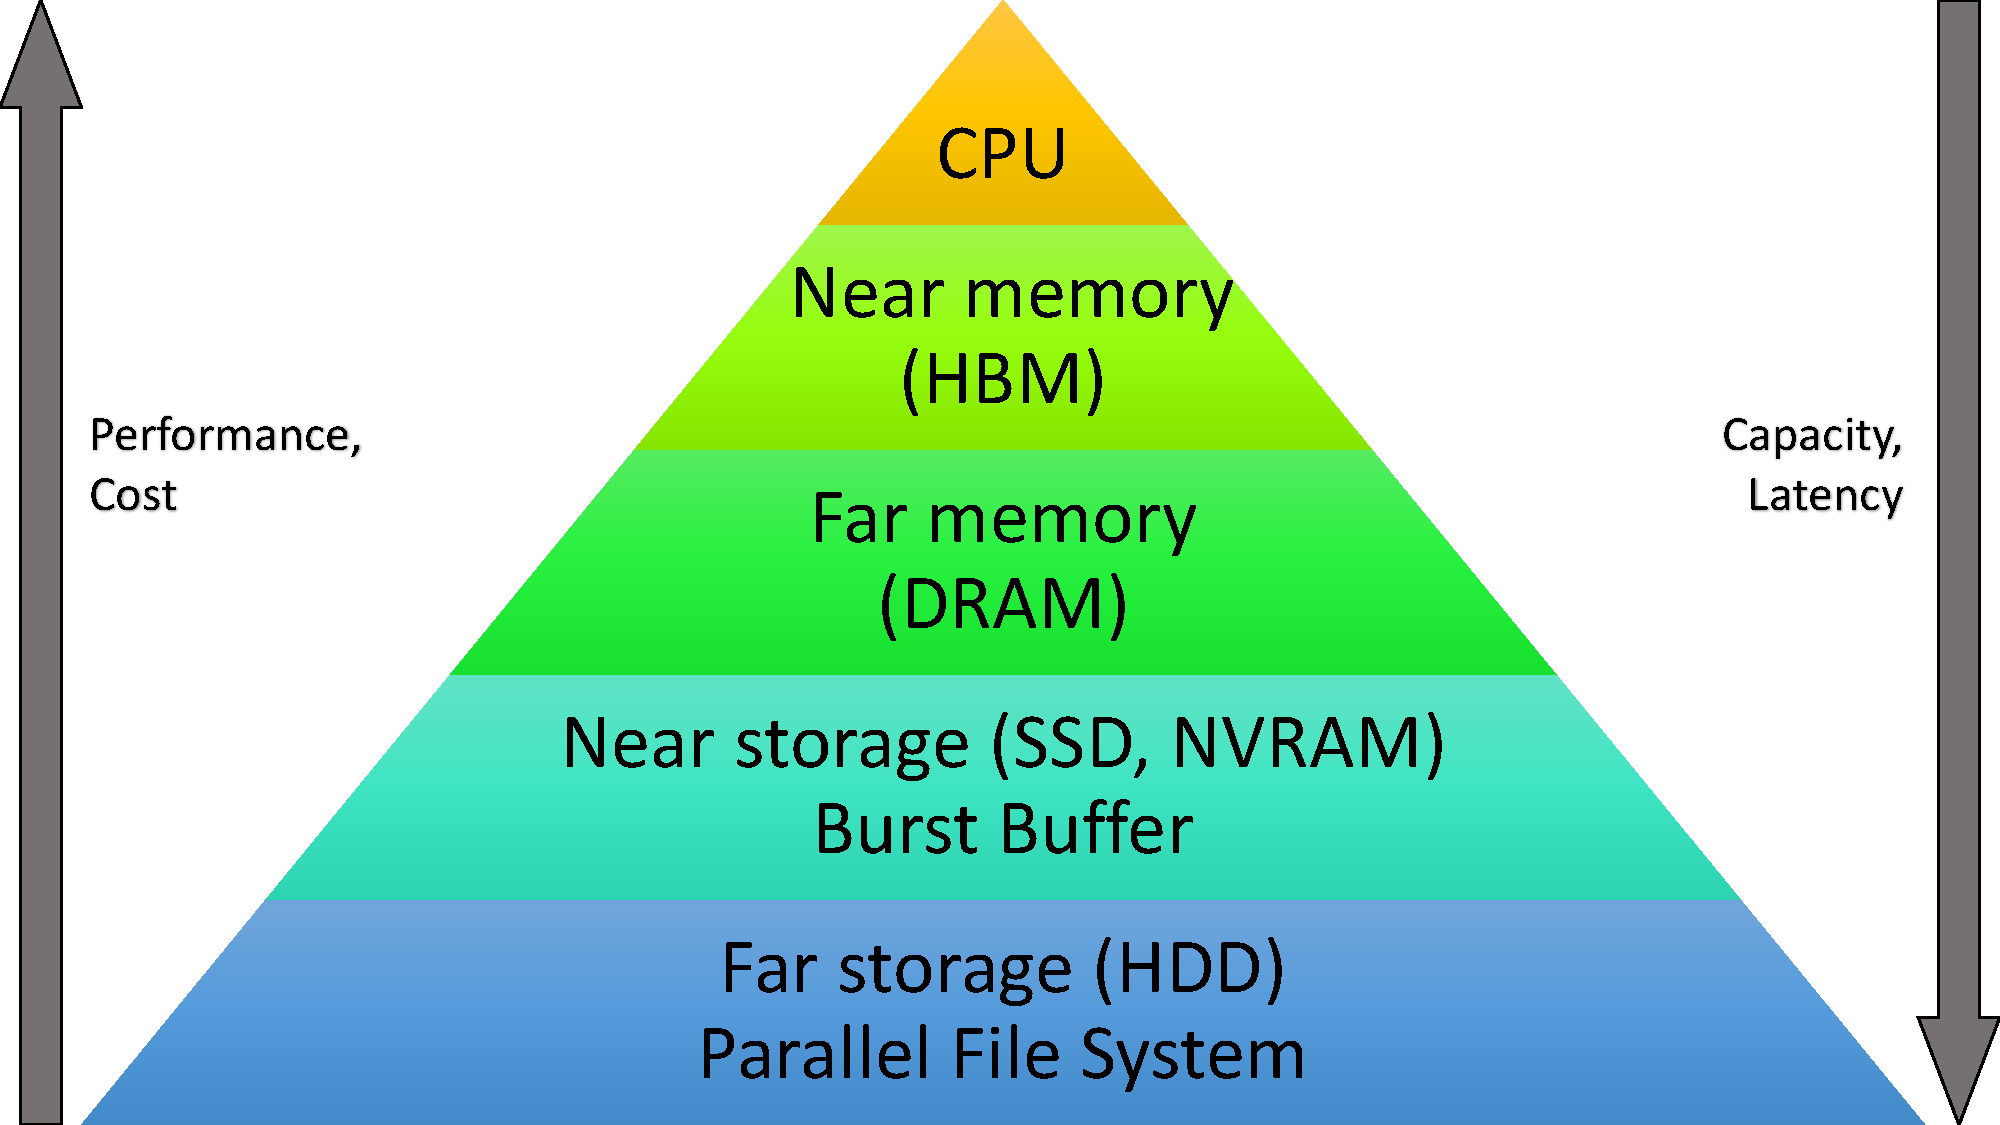
\includegraphics[width=\textwidth]{images/Memory-hierarchy.pdf}
    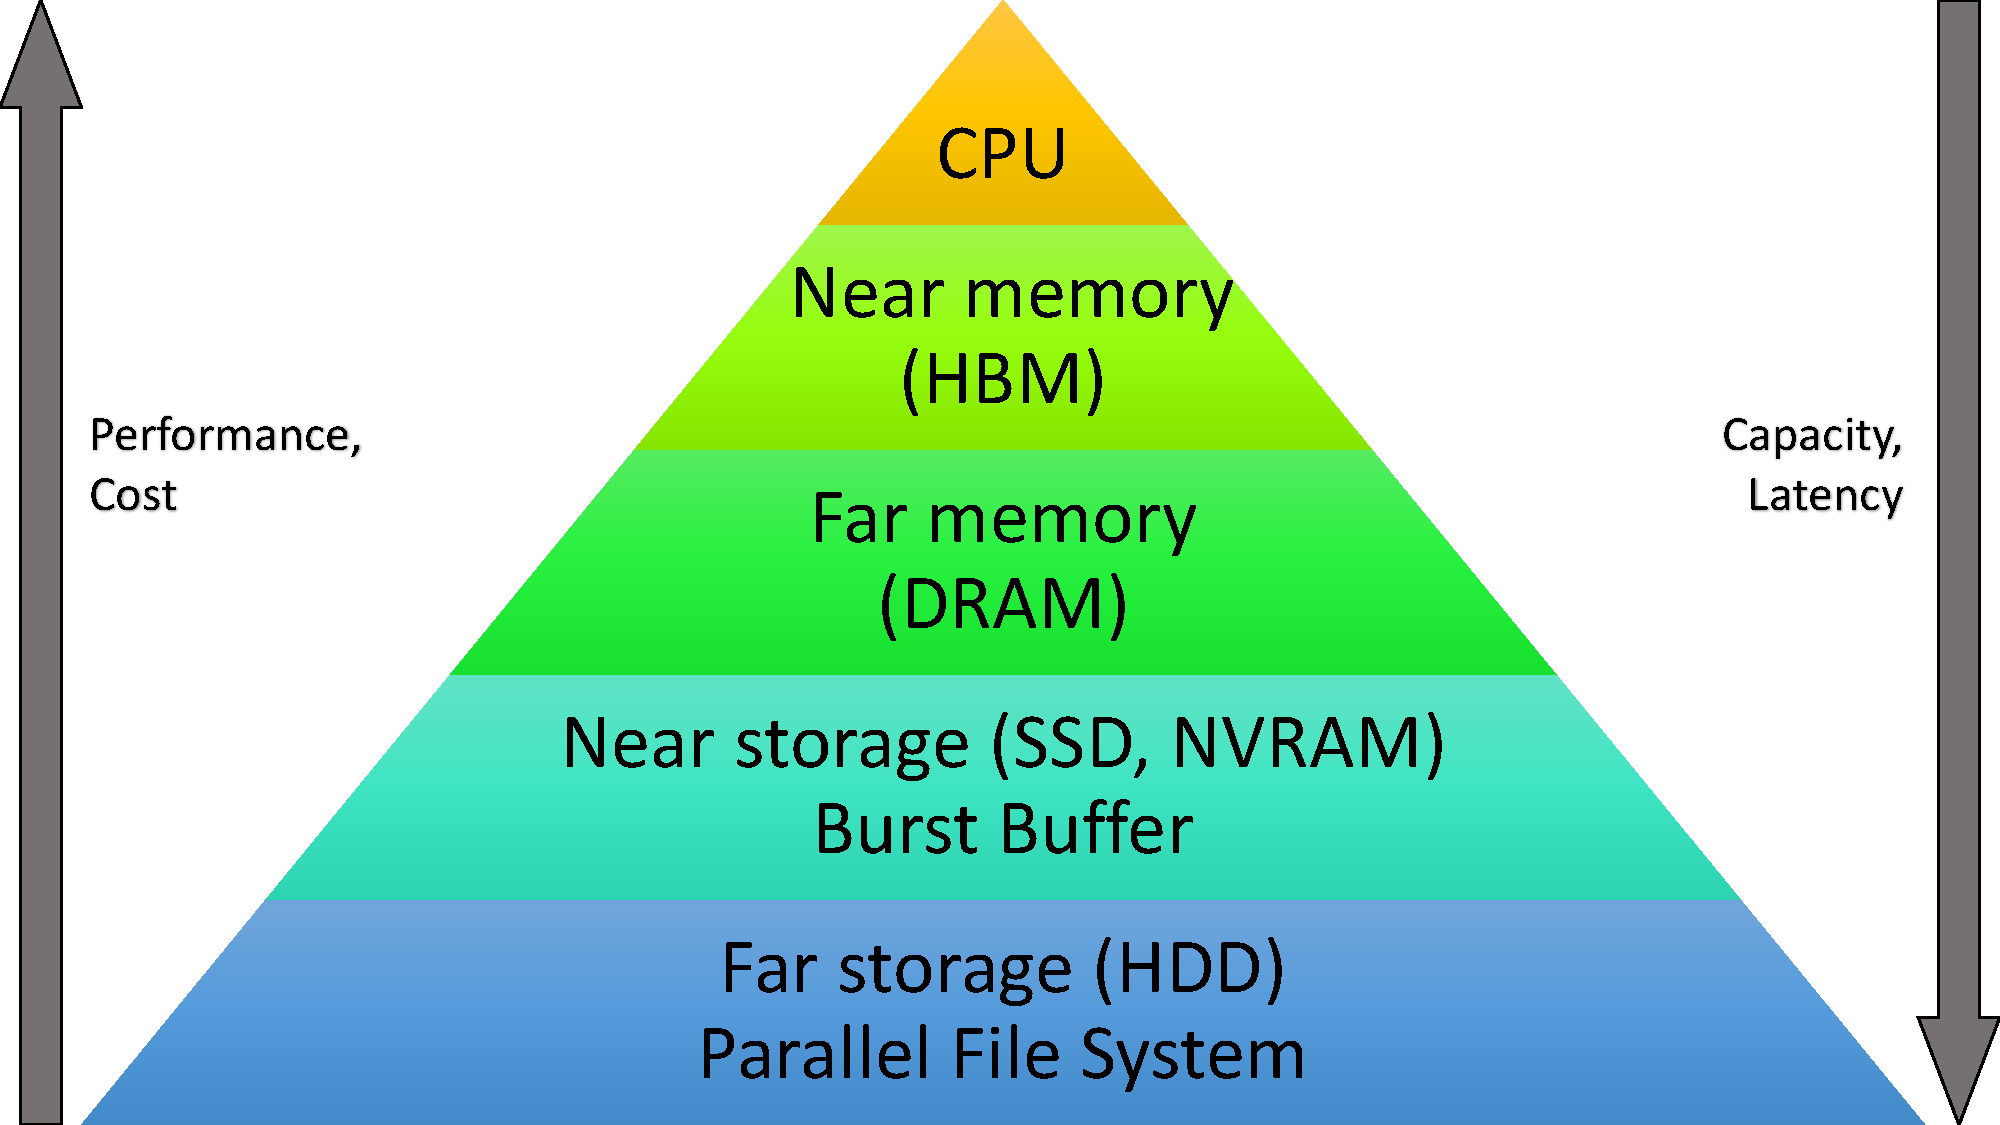
\includegraphics[width=0.9\textwidth]{images/Memory-hierarchy.pdf}
    \caption{Memory hierarchy of a modern supercomputer with burst buffers}
    \label{fig:memory-hierarchy}
\end{figure}

\section{Far storage in a Parallel File System}
A parallel file system (PFS), also known as a clustered file system, is a type of file system designed to store data across multiple networked servers and to facilitate high-performance access through simultaneous, coordinated input/output operations between parallel applications running on compute nodes and storage nodes. PFS is usually deployed on the backend storage (far storage, long-term storage) of supercomputers and HPC clusters.

PFS breaks up a dataset and distributes/stripes blocks to multiple storage drives, which can be located in local or remote servers. Users do not need to know the physical location of the data blocks to retrieve a file, as the system uses a global namespace to facilitate data access. Data is read and written to the storage devices using multiple I/O paths concurrently, which provides a significant performance benefit. Storage capacity and bandwidth can be scaled to accommodate enormous quantities of data. Features of PFS may include high availability, mirroring, replication and snapshots.

Throughout this work, we will use the term PFS interchangeably with the backend storage system.

\section{Burst buffer use cases}
The primary motivation for the existence of burst buffers was to absorb the periodic I/O bursts of HPC applications, especially increasing the performance of periodic checkpoints. However, burst buffers bring several additional use cases that may increase the performance of individual applications or a whole HPC system. Based on the gathered literature \cite{osti_1328312,bhimji2016accelerating,6232369,8891051,10.5555/3108096.3108100,romanus2015challenges,lockwood-blog} we selected common use cases of burst buffers.

\paragraph{Periodic I/O bursts}
Scientific applications' I/O patterns are often characterised by enormous spikes in I/O traffic, which is due to their life cycles that typically alternate between computation phases and I/O phases. In other words, after each round of computation, all computing processes concurrently write their intermediate data to backend storage systems. This pattern is then repeated with another round of computation and data movement operations. 

Traffic to PFS is often mostly limited by slow hard drives as well as bandwidth and contention of storage network. As a consequence, the significant I/O bursts are causing high I/O latency of application and under-utilisation of computing resources.

With the deployment of burst buffers, applications can quickly write their data to a burst buffer after a round of computations instead of writing to the slow hard disk--based storage systems. Therefore, they receive a quick confirmation of data being saved in persistent memory and may proceed to the next round of computations without waiting for the data to be moved to the slow backend storage systems. The data stored in burst buffers are then asynchronously flushed to the PFS, which overlap with the next round of computation. In this way, the extended I/O time spent in moving data to the storage systems is hidden by the computation time.

\paragraph{Checkpoint/restart}
One complexity in HPC is that an interruption of any process of a parallel application destroys the distributed state of the entire application. As the number of nodes in supercomputers constantly increases, the size of the distributed state grows. To ensure forward progress parallel applications use checkpoints to allow a job to restart from an intermediate state in case of a failure. That is a conceptually simple technique of persisting their distributed state at regular time intervals and avoiding repetition of all computations.

\paragraph{Data staging}
Stage-in and stage-out is a technique of moving input and output data of an application from PFS to burst buffers. The key concept is to make the input data available in the fast storage, close to compute resources, rather than slow backend storage. In the naive approach, data staging could take place immediately when a job starts. However, as compute resources are not necessary for data moving, the stage-in phase of one application could be overlapped with computations of another application that was previously allocated with a set of computing resources shared with the first application. Similarly, the stage-out from a burst buffer could allow flushing of output data to PFS after freeing of computing resources. In result, this technique could improve the overall utilisation of a supercomputing system. According to \cite{osti_1544343} stage-in and stage-out with burst buffers are used in the following scientific applications: SWarp and CAMP (Community Access MODIS Pipeline).

\paragraph{Write-through cache}
A write-through cache is a caching technique in which data is simultaneously copied to cache and to backend storage systems. It allows to increase the read performance as data is already available in fast storage, which may be gradually synchronised with far persistence storage. The urge to make the caching as easy as possible from the application perspective implies attempts to implement write-through cache in the form of the transparent caching mode. For instance, both Data Direct Network's Infinite Memory Engine and Cray DataWarp systems implement the transparent caching mode \cite{lockwood-blog}.

\paragraph{Data sharing}
Burst buffers may be applied to enable data sharing within and across applications. An application could utilise burst buffers to create a shared file and use it to communicate among compute nodes. Different I/O models may be applied for this purpose, such as one-file--per-job (N-1), file-per-process (N-N) or more complex patterns (N-M). These models were discussed in \cite{7877147,6375580}.

Burst buffers may also be used to enable data sharing between consecutive jobs. A scientific workflow may be divided into several stages, each performed as a separate job. In this scenario, intermediate data passed between jobs may be persisted in a burst buffer instead of sending it back and forth to PFS.

\paragraph{In-situ analysis}
An in-situ analysis is a type of data analysis and visualisation that happen concurrently to the main computational task. Burst buffers are utilised here to store data and perform analysis without data movement to PFS. The kind of data subject to analysis may be an application checkpoint.

\paragraph{Out-of-core memory}
For applications for which available main memory (DRAM) is not enough, non-volatile devices may be used to extend the application memory. NVDIMM is the type of NVM hardware that could provide adequate performance for this use case. Installed on a compute node it can be configured either as extended main memory or a burst buffer.

\section{Overview of non-volatile memory hardware}
A burst buffer is a concept of a fast, non-volatile, intermediate storage layer logically positioned between dynamic random-access memory (DRAM) in compute nodes and a parallel file system. DRAM, which colloquially referred to as RAM, is a type of a fast, volatile memory that serves the role of primary storage. It is widely used in most of the modern devices such as personal computers, mobile devices and server machines. Volatility in the context of memory means that it requires power to maintain stored information. Once the power of volatile memory is down, stored data is quickly lost. In contrast, the non-volatile memory (NVM) is persistent even if not continuously supplied with electric power.

The term NVM refers to a wide variety of memory types. Examples of these include flash memory, read-only memory (ROM), floppy disks, optical discs, hard disk drives (HDD), solid-state drives (SSD), Non-volatile random-access memory (NVRAM) and many others. All of these memory types are characterised by the ability to retain data without applied power. The types of NVM used as burst buffers in supercomputer architectures are SSD and NVRAM. The reason for this is that they offer a much higher performance of data access compared to other persistent memory types.

\paragraph{Solid State Drive}
SSDs are usually constructed with the use of non-volatile NAND flash memory. Another type of hardware architecture is a DRAM-based SSD, which is a DRAM supplied with an additional source of power such as an internal battery. When external power is lost, the battery provides power, and all data is copied to a persistence backup storage. There also exists a new NVM technology called 3D XPoint announced by Intel and Micron. It could be used both as an ordinary SSD or as NVDIMM (non-volatile dual in-line memory module). SSDs with the 3D Xpoint technology is currently available on the market as Intel Optane SSDs and Micron QuantX X100.

% Solid State Drives are used in the following supercomputers:
% \begin{itemize}
% \item Fugaku at the RIKEN Center for Computational Science - about 1.6 TB SSD \cite{fugaku}
% \item Summit at the Oak Ridge National Laboratory - 1.6 TB Samsung NVMe SSD \cite{osti_1489443}
% \item Sierra at the Lawrence Livermore National Laboratory - 1.6 TB Samsung NVMe SSD \cite{osti_1489443}
% \item Tsubame at the Tokyo Institute of Technology - Intel DC P3500 2TB (NVMe, PCI-E 3.0 x4, R2700/W1800) \cite{tsubame}
% \item Theta at the Argonne National Laboratory - Samsung SM961 MZVPV128HEGM (128 GB) \cite{theta-fs}
% \item Tianhe-2 at the National Supercomputer Center in Guangzhou - 1TB PCIe SSD \cite{tianhe}
% \item Trinity at the Los Alamos National Laboratory - 4 TB Intel P3608 (PCI-E x4) \cite{trinity,osti_1367056}
% \end{itemize}

\paragraph{Non-volatile RAM}
As there is no standardised definition of NVRAM, this term is often ambiguous and interchangeably used with NVM, NVDIMM, DRAM-based SSD and NAND-based SSD. Particularly, ordinary SSDs based on NAND-Flash memory are frequently referred to as NVRAM, for instance in \cite{osti_1544343}. NEXTGenIO, an initiative supporting the development of Intel Optane DC Persistent Memory in supercomputing, defines NVRAM as memory \textquote{implemented by NVDIMMs, being one kind of NVM, that supports both non-volatile RAM access and persistent storage} \cite{nextgenio}. NVDIMM is a non-volatile random-access memory in the form of a DIMM package, which is a mainstream pluggable form factor for DRAM. Development of NVRAM in the form of NVDIMM raises the potential of using it as a system's main memory.
% We follow the definition of the NEXTGenIO

Historically, there have been numerous different approaches to implementing NVRAM. The modern solutions in implementing NVRAM in hardware include:
\begin{itemize}
\item Ferroelectric RAM,
\item Magnetoresistive RAM,
\item Phase-change RAM,
\item Millipede memory,
\item FeFET memory.
\end{itemize}
Out of these solutions, Magnetoresistive RAM (MRAM) and Phase-change RAM (PRAM) are currently in commercial production. An example of PRAM-based solution is the 3D XPoint technology. Intel develops a family of devices based on this technology under the trademark of Intel Optane. The NVRAM devices are offered as Intel Optane Persistent Memory. Everspin is the company specialised in MRAM-based solutions. It produces a variety of MRAM devices including the advanced STT-MRAM technology.

% As NVRAM is still an emerging technology in supercomputing, it is not commonly used for implementing burst buffers. According to publicly available online sources, currently, it is available at:
% \begin{itemize}
% \item Cori at the Lawrence Berkeley National Laboratory \cite{cori, cori-exp, bhimji2016accelerating, Bhimji_2017}
% \item Catalyst at the Lawrence Livermore National Laboratory \cite{catalyst}
% \end{itemize}

\bigskip

The following list gathers supercomputers equipped with burst buffers together with the information about their NVM devices. The citation in each entry refer to the source of the information.
\begin{itemize}
\item Fugaku at the RIKEN Center for Computational Science - about 1.6 TB SSD \cite{fugaku,dongarra2020report}
\item Summit at the Oak Ridge National Laboratory - 1.6 TB Samsung NVMe SSD \cite{osti_1489443}
\item Sierra at the Lawrence Livermore National Laboratory - 1.6 TB Samsung NVMe SSD \cite{osti_1489443}
\item Tsubame at the Tokyo Institute of Technology - 2 TB Intel DC P3500 (NVMe, PCI-E 3.0 x4, R2700/W1800) \cite{tsubame}
\item Theta at the Argonne National Laboratory - 128 GB Samsung SM961 MZVPV128HEGM SSD \cite{theta-fs}
\item Tianhe-2 at the National Supercomputer Center in Guangzhou - 1 TB PCIe SSD \cite{tianhe}
\item Trinity at the Los Alamos National Laboratory - 4 TB Intel DC P3608 NAND flash SSD \cite{trinity,osti_1367056}
\item Cori at the Lawrence Berkeley National Laboratory - 3.2 TB Intel DC P3608 NAND flash SSD (described as NVRAM) \cite{cori, cori-exp, bhimji2016accelerating, Bhimji_2017}
\item Catalyst at the Lawrence Livermore National Laboratory - 800 GB Intel SSD 910 (described as NVRAM) \cite{catalyst,7573843}
\end{itemize}

\section{Burst buffers in supercomputer architectures} \label{sec:architectures}
At the top most level of burst buffer placement classification in supercomputer architectures, there could be distinguished two architectures: node-local and remote shared burst buffers. The node-local burst buffer is a well-established term, which appears in numerous papers \cite{8891051,10.5555/3108096.3108100,osti_1328312}. The remote shared burst buffers could be further divided depending on their placement in a supercomputer. Khetawat \textit{et al.} \cite{8891051} distinguished shared burst buffers between grouped and global. Another terminology is introduced in the Oak Ridge National Laboratory technical report by Harms \textit{et al.} \cite{osti_1328312}. They classified burst buffer architectures into compute node--local storage, co-located with I/O nodes and the last kind using a separate set of nodes. Glenn K. Lockwood proposed the most granular division on his blog \cite{lockwood-blog}, where he distinguished the architectures between compute node attached, I/O node attached, fabric attached and storage fabric attached.

All of the architectures described below, except the hybrid, are presented in \autoref{fig:burst-buffer-architectures}.

\begin{figure}[htb] 
  \begin{subfigure}[b]{0.5\linewidth}
    \centering
    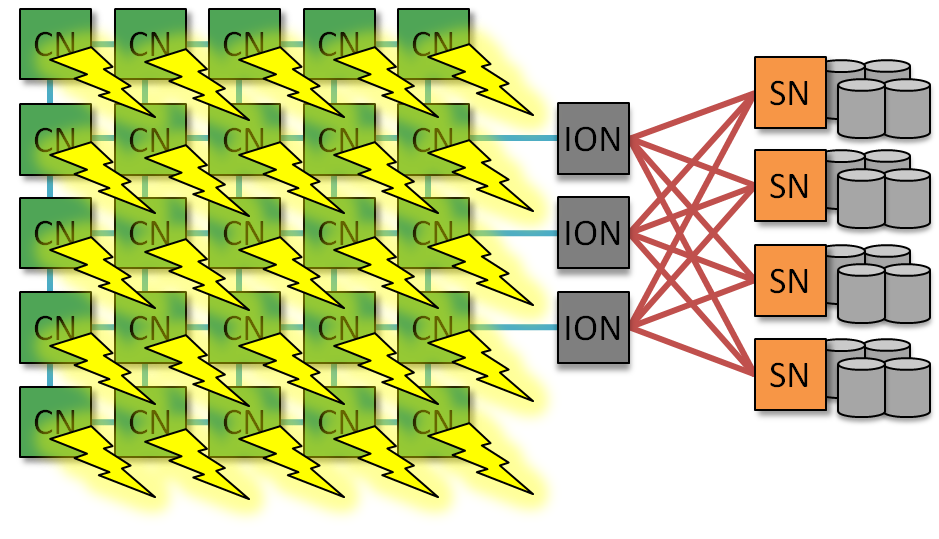
\includegraphics[width=0.8\linewidth]{images/architecture-on-cn.png} 
    \caption{Node-local burst buffers} 
    \label{fig:architecture-on-cn} 
    \vspace{4ex}
  \end{subfigure}
  \hfill
  \begin{subfigure}[b]{0.5\linewidth}
    \centering
    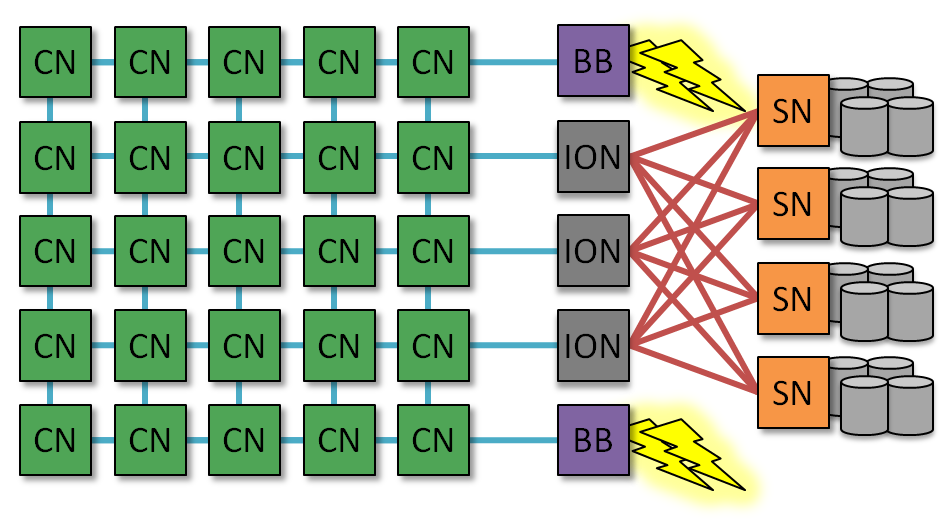
\includegraphics[width=0.8\linewidth]{images/architecture-on-edge.png} 
    \caption{Compute network-attached burst buffers} 
    \label{fig:architecture-on-edge}
    \vspace{4ex}
  \end{subfigure} 
  \begin{subfigure}[b]{0.5\linewidth}
    \centering
    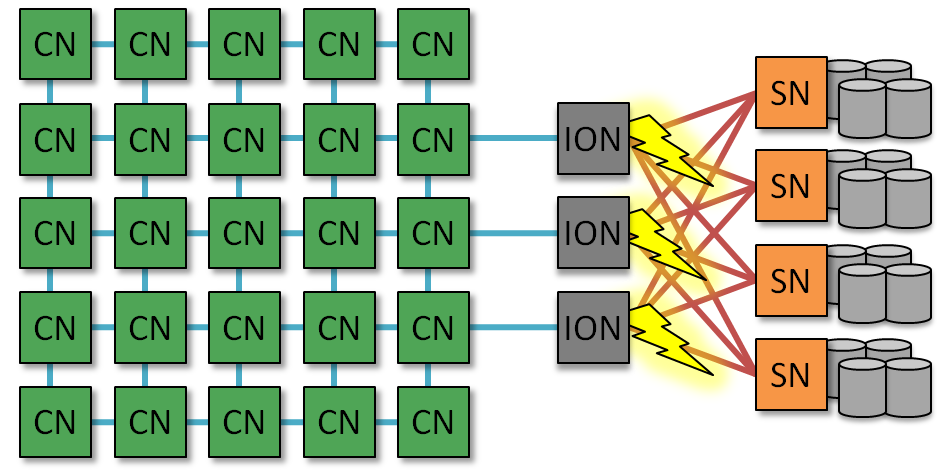
\includegraphics[width=0.8\linewidth]{images/architecture-on-ion.png} 
    \caption{Burst buffers co-located with I/O nodes} 
    \label{fig:architecture-on-ion} 
  \end{subfigure}
  \hfill
  \begin{subfigure}[b]{0.5\linewidth}
    \centering
    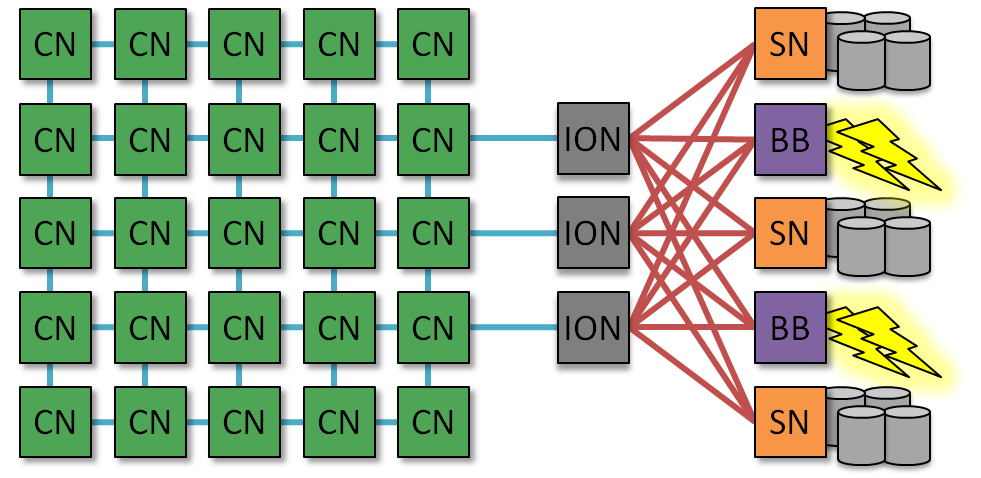
\includegraphics[width=0.8\linewidth]{images/architecture-backend.png} 
    \caption{Storage network-attached burst buffers} 
    \label{fig:architecture-backend} 
  \end{subfigure} 
  \captionsource{Illustration of various burst buffer architectures (CN - compute node, ION - I/O node, SN - long-term storage node, BB - dedicated burst buffer node, lightning - burst buffer placement).}
  {\url{https://glennklockwood.blogspot.com/2017/03/reviewing-state-of-art-of-burst-buffers.html}}
  \label{fig:burst-buffer-architectures} 
\end{figure}

\paragraph{Node-local burst buffers}
In the compute node-local burst buffer architecture, burst buffer storage is located on each compute node. The main advantage of this architecture is a performance scaling. The aggregate burst buffer bandwidth scales linearly with the number of compute nodes, which has been confirmed, for example in \cite{Wang2016BurstFSAD,5645453}. Another benefit is exclusive and fair access of applications to the storage devices, which provides more consistent and predictable access to storage resulting in lower variation in I/O performance. Further, during application I/O, there is no network traffic, and the large reads or writes do not impact any shared resources such as network or PFS. This architecture is also interface-free, meaning that an operating system can create a local POSIX file system on a burst buffer and applications can use a standard software storage stack.

However, there are several disadvantages of node-local architecture. First of all, there is limited support for shared-file I/O as individual burst buffers are not shared between compute nodes. Consequently, standard file access techniques, such as many readers or writers sharing a single file, called the N-1 model, are difficult to implement. They require an additional I/O middleware. Further, stage-in and stage-out require network traffic to the compute nodes. Another drawback of using this storage model is that the burst buffers are tightly coupled with the compute nodes, which creates a single failure domain. Lastly, any maintenance required by the storage device may demand taking the entire compute node offline.

This architecture was deployed in several systems, including the Summit and Sierra, which are the second and third top supercomputers (as of June 2020) \cite{top500}. The more comprehensive list is presented below:
\begin{itemize}
\item Summit at the Oak Ridge National Laboratory \cite{osti_1489443}
\item Sierra at the Lawrence Livermore National Laboratory \cite{osti_1489443}
\item Tsubame at the Tokyo Institute of Technology \cite{tsubame}
\item Theta at the Argonne National Laboratory \cite{theta-fs}
\end{itemize}

% \begin{figure}[h]
%     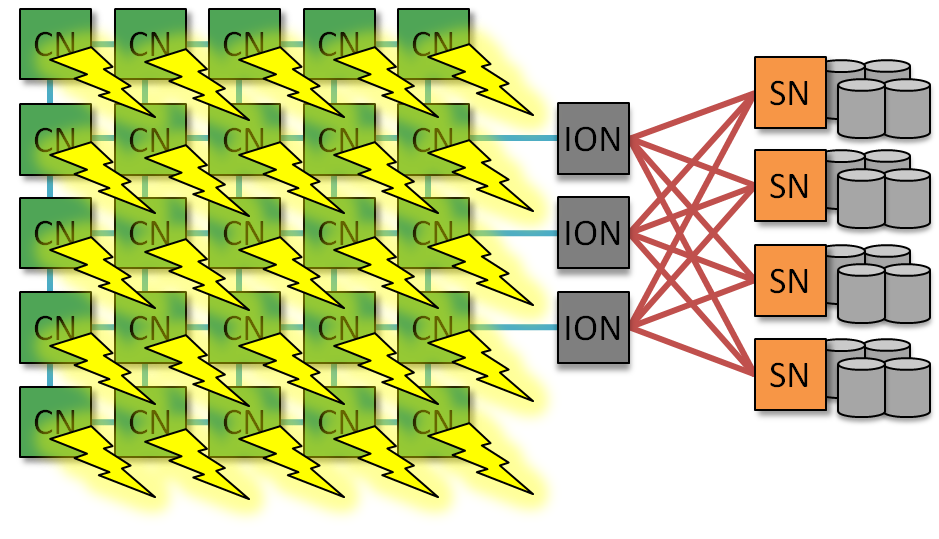
\includegraphics[width=\textwidth]{images/architecture-on-cn.png}
%     \captionsource{Node-local burst buffers.}
%     {\url{https://glennklockwood.blogspot.com/2017/03/reviewing-state-of-art-of-burst-buffers.html}}
%     \label{fig:architecture-on-cn}
% \end{figure}

\paragraph{Burst buffers co-located with I/O nodes}
I/O nodes are networking element that route data between compute fabric and backend storage fabric. The I/O nodes could be either commodity routers or specialised forwarding devices.

The positioning of SSDs or NVRAM devices within I/O nodes results in the shared burst buffer architecture, which may readily support N-1 and N-N communication models. Possibly, it is the easiest to realise data staging (stage-in and stage-out) is in this architecture as it might not require any traffic to the compute network. This architecture also provides data resiliency and longer residency times than node-local burst buffers. 

There are yet some drawbacks of burst buffers co-located with I/O nodes. Firstly, as storage resources are shared among compute nodes, this might lead to interference among application resulting in unpredictable performance. Secondly, the compute network connections are shared between burst buffer and PFS traffic, which would negatively impact PFS performance at an occurrence of bursty I/O. Furthermore, the storage capacity scalability of this architecture is limited by a fixed number of I/O nodes. The most significant concern of incorporating burst buffers into I/O nodes are maintenance and failure dependency between them.

The architecture of burst buffers co-located with I/O nodes was deployed in the Tianhe-2 system at the National Supercomputer Center in Guangzhou \cite{tianhe}.

% \begin{figure}[h]
%     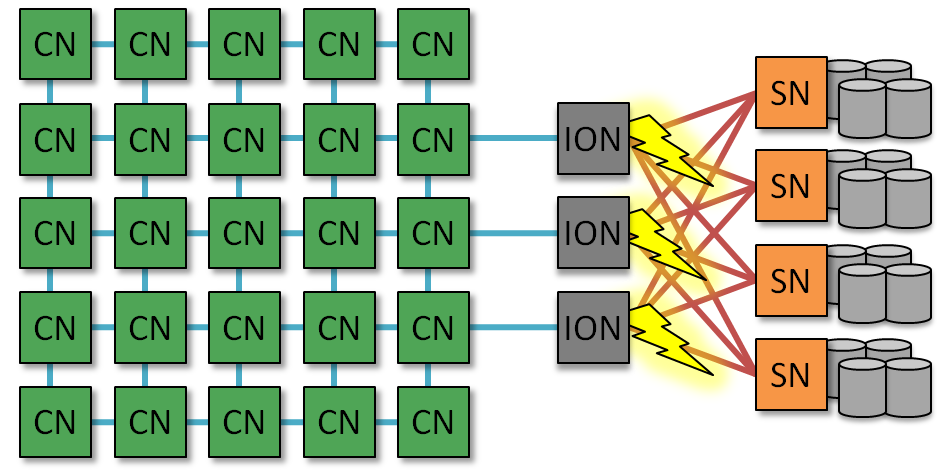
\includegraphics[width=\textwidth]{images/architecture-on-ion.png}
%     \captionsource{Burst buffers co-located with I/O nodes.}
%     {\url{https://glennklockwood.blogspot.com/2017/03/reviewing-state-of-art-of-burst-buffers.html}}
%     \label{fig:architecture-on-ion}
% \end{figure}

\paragraph{Compute network-attached burst buffers}
This design places burst buffers in dedicated nodes within a compute network. Location of these nodes may vary, resulting in different proximity between a compute node and PFS. For instance, a single node of every chassis or cabinet could be dedicated to be a burst buffer. Another approach is to create special storage nodes directly connected with the I/O nodes. This architecture inherits most of the advantages of burst buffers co-located with I/O nodes, including easy data sharing, support for N-1, N-N models, longer residency times and data resiliency. The principal additional advantage of separate dedicated nodes is the transparent maintenance of a supercomputing cluster. SSDs are characterised by a limited number of write operations, which creates a necessity of replacing them over time. Having a separate burst buffer nodes enables to maintain them without downtime of compute or I/O nodes. Conversely, it also provides a possibility of continued use when an I/O node or PFS goes offline. 

Similarly to co-location with I/O nodes, compute network-attached burst buffers are burdened with application interference in shared network connection. Furthermore, this architecture brings the highest price cost due to the cost of additional servers and network infrastructure.

Two dedicated hardware and software production systems were created following this burst buffer architecture: Cray DataWarp and Infinite Memory Engine developed by Data Direct Network. The Cray DataWarp was deployed in the Cori system at the Lawrence Berkeley National Laboratory \cite{cori-exp, bhimji2016accelerating, Bhimji_2017}, which architecture schema is presented in \autoref{fig:cori-architecture} and Trinity at the Los Alamos National Laboratory \cite{trinity,osti_1367056}.

Currently, the fastest supercomputer in the world according to TOP500 list \cite{top500}---Fugaku at the RIKEN Center for Computational Science---utilises a shared burst buffer architecture with SSDs in one of every 16 compute nodes \cite{fugaku}.

\begin{figure}[htb]
    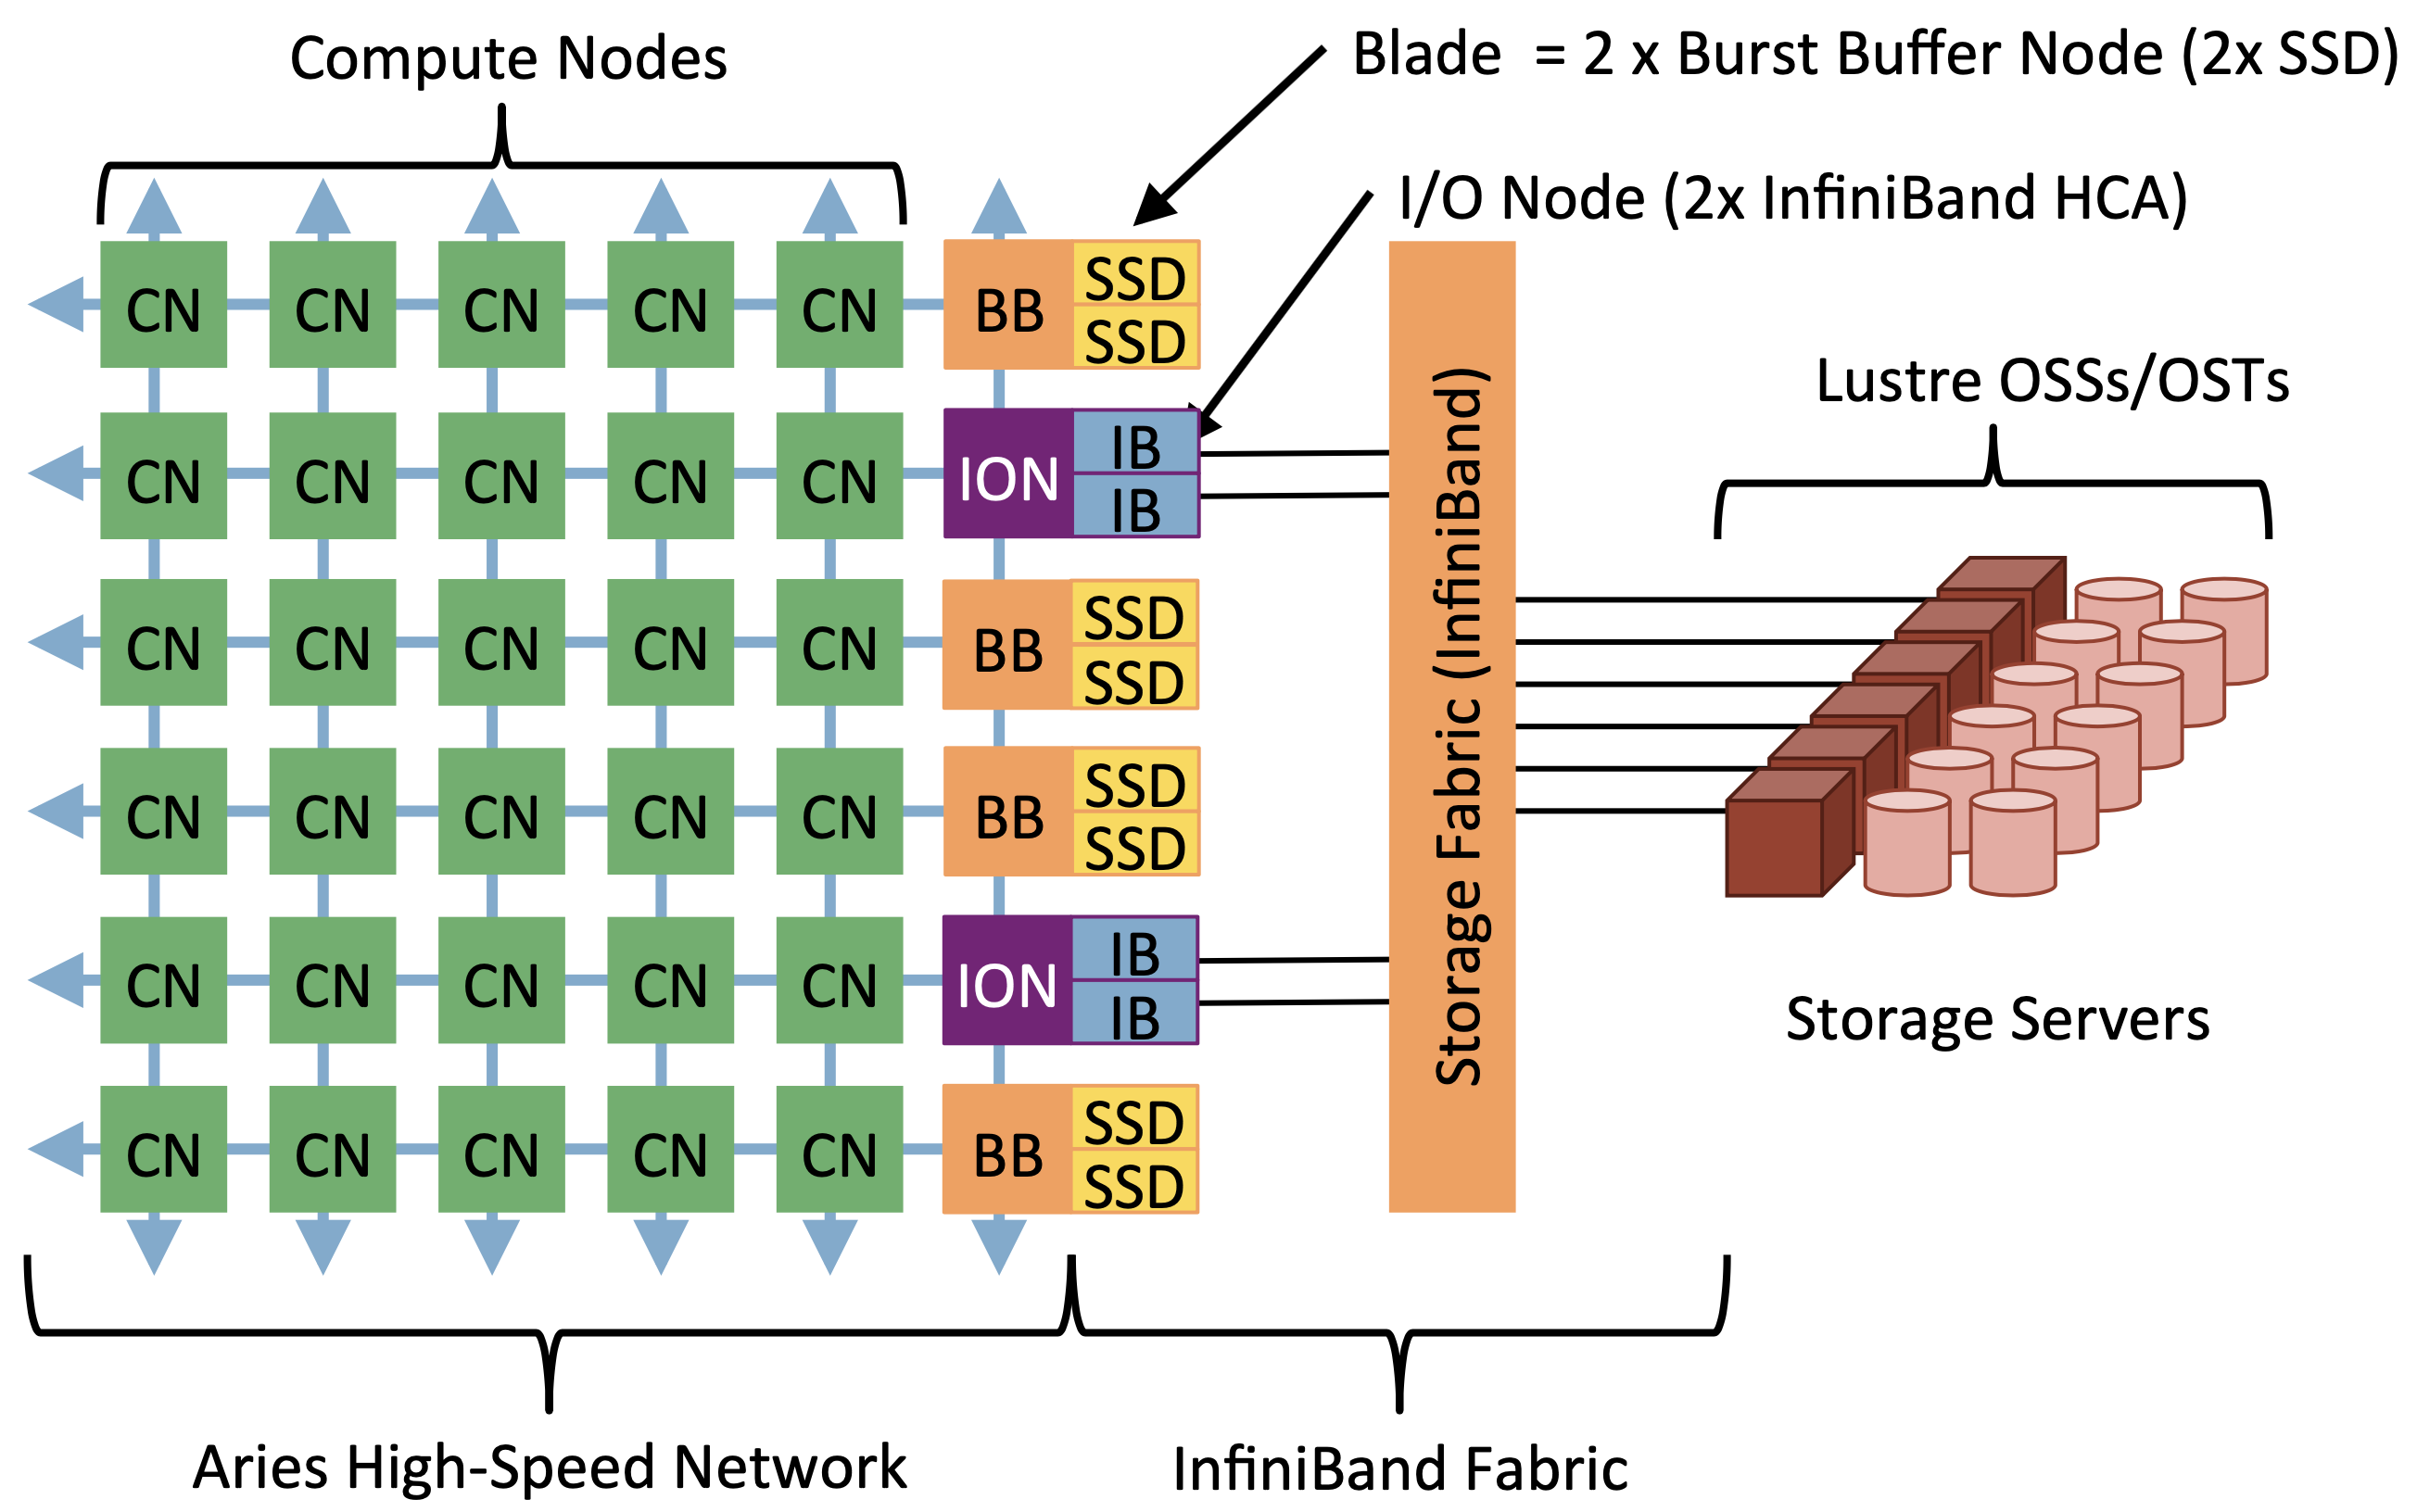
\includegraphics[width=\textwidth]{images/cori-architecture.png}
    \captionsource{The placement of the burst buffer nodes in the Cori System}
    {Accelerating Science with the NERSC Burst Buffer Early User Program \cite{bhimji2016accelerating}}
    \label{fig:cori-architecture}
\end{figure}
% \begin{figure}[h]
%     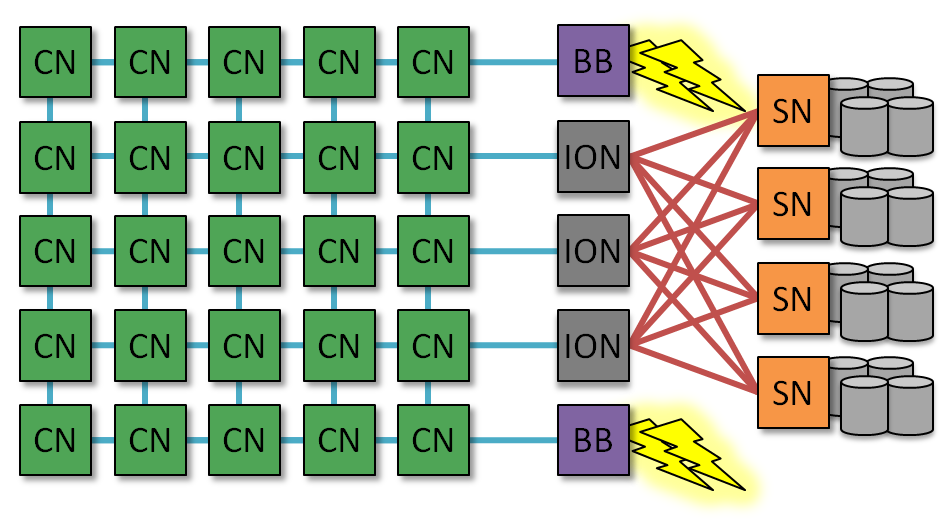
\includegraphics[width=\textwidth]{images/architecture-on-edge.png}
%     \captionsource{Network-attached burst buffers.}
%     {\url{https://glennklockwood.blogspot.com/2017/03/reviewing-state-of-art-of-burst-buffers.html}}
%     \label{fig:architecture-on-backend}
% \end{figure}

\paragraph{Backend storage network-attached burst buffers}
The last of fundamental architectures involves attaching NVM devices to a storage network, either as fast storage on the nodes hosting long-term storage or as a separate set of nodes. This model creates an off-platform burst buffer, which may not provide the highest absolute performance, but may provide significant ease of use benefits via transparent caching.  HPC systems with custom compute fabrics are the primary reason for the use of this design as they are usually not amenable to adding third-party burst buffers.

% Long term storage
% \begin{figure}[h]
%     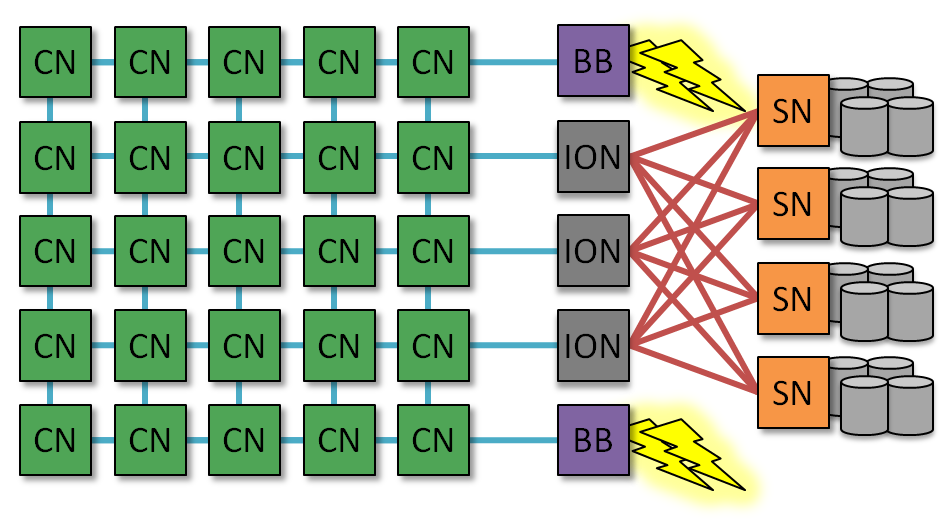
\includegraphics[width=\textwidth]{images/architecture-on-edge.png}
%     \captionsource{Long-term storage network-attached burst buffers.}
%     {\url{https://glennklockwood.blogspot.com/2017/03/reviewing-state-of-art-of-burst-buffers.html}}
%     \label{fig:architecture-backend}
% \end{figure}

\paragraph{Hybrid architecture}
It is also possible to mix the described architectures creating a multi-level heterogeneous storage model. A particularly interesting variation would be a mixture of node-local burst buffers with NVRAM and dedicated network-attached nodes directly connected to I/O nodes, equipped with SSDs. Such an architecture could handle applications with distinct I/O patterns and offer both high performance, exclusive access to permanent storage as well as support for shared I/O models. Software solutions that transparently move data across multiple storage layers have already been explored in \cite{8514867,8411015,10.1145/3208040.3208059}.

\section{Resources and Jobs Management Systems} \label{sec:rjms}
Resource and Jobs Management Systems (RJMS) are complex middlewares, which are the core of platform management and serve several roles. First, they receive job submissions from users and allocate exclusive or non-exclusive access to platform resources (compute nodes, accelerators, memory, burst buffers) for some duration of time, which could be shortly described as management of resource sharing. Second, it provides a framework for starting, executing, and monitoring (usually parallel) jobs on the set of allocated resources. Finally, it arbitrates contention for resources by managing a queue of pending jobs.

RJMSs are therefore the place to take management decisions and to implement management policies and algorithms, hence are often abbreviated as merely---job scheduler or batch scheduler. Despite being commonly called as batch schedulers, they usually support submission of both batch and interactive jobs. RJMSs, besides of functional requirements, are also required to satisfy multiple non-functional requirements such as fault-tolerance, high scalability, fair resource sharing.

The well-known job schedulers in HPC include Slurm \cite{10.1007/10968987_3,slurm}, Moab/TORQUE \cite{moab-torque}, PBS \cite{pbs-pro,open-pbs}, and Flux \cite{flux}.

\section{Scheduling algorithms} \label{sec:algorithms}
As described in \autoref{sec:rjms}, one of the key aspects of RJMSs is queuing and scheduling of jobs given available resource in a platform. For this matter, multiple algorithms were created out of which the most fundamental are FCFS, aggressive and conservative backfilling. We summarise these methods based on the information and observations gathered in \cite{srinivasan2002characterization,srinivasan2002selective,feitelson2005experimental,8752660}. It is also valuable to distinguish between online and offline scheduling. In online scheduling, new jobs may arrive during the execution of a workload, whereas in offline, all jobs are available for scheduling at the same point of time.

In the existing schedulers, processors are the primary resources that are subject to scheduling. All other resources, such as main memory, are secondary. Batch schedulers were designed to optimise the system utilisation of processors, while the availability of other resources is just a constraint for scheduling, such as the main memory in compute nodes.

In the field of scheduling in HPC systems, jobs are often considered to be parallel, rigid and non-preemptive. The parallelism of jobs means that they run on multiple processors simultaneously, where processors are either compute nodes, CPUs or CPU cores depending on the context. The non-preemptive character states that running jobs cannot be interrupted and interleaved with each other. Rigid jobs are jobs that specify the number of processors they need and run for a particular time using this number of processors. Scheduling of parallel jobs is usually viewed in terms of a 2D chart with time along one axis and the number of processors along the other axis. Each job can be then depicted as a rectangle whose length is the user estimated runtime and width is the required number of processors. This 2D chart is a special kind of a Gantt chart. In particular, it is commonly used to visualise executed jobs in batch job scheduling. \autoref{fig:reservation_alloc-only_gantt_future_head} is an example of the Gantt chart.

Based on the shape of those rectangles, jobs could be classified into four categories. Two basic classes are derived from the runtime of jobs: short and long. Two other classes are orthogonal to runtime and are based on the number of processors requested: narrow (serial and small jobs) and wide (jobs with a large number of processors). With these classes combined, jobs could be categorised into short-narrow, short-wide, long-narrow and long-wide. The distinction between short and long as well as narrow and wide jobs is subject to a concrete problem statement, computing cluster and workload. An example of a specific quantitative definition may be found in \autoref{sec:bbrequest}.

\subsection{Queuing policies}
The job queue, into which jobs arrive, could be a priority queue and implement various priority policies.

The most straightforward scheduling policy is First-Come-First-Served (FCFS), where jobs are executed in the order of their arrivals whenever enough of the resources is available. Although this is a fair policy of resource sharing, this approach suffers from low system utilisation.

Another popular policy is Shortest Jobs First (SJF), a.k.a. Shortest estimated Processing time First (SPF), according to which the jobs are sorted in ascending order based on the estimated running time. There are also the Smallest Requested Resources First (SQF) and Smallest estimated Area First (SAF).

\subsection{Backfilling}
Backfilling works by identifying holes between jobs (rectangles) in the 2D chart and moving forward smaller jobs that fit these holes. As described at the beginning of \autoref{sec:algorithms}, this 2D chart is a special kind of a Gantt chart. In order to avoid starvation of large jobs, jobs at the front of a waiting queue are assigned reservations of resources with associated start times. Other jobs are not permitted to use the reserved resources.

\paragraph{Conservative backfilling}
In the conservative backfilling, each job is given a reservation when it arrives to the queue, and jobs are allowed to move ahead in the queue as long as they do not cause any queued job to get delayed beyond their reserved start time. In other words, a newly arriving job is given the reservation at the earliest time that will not violate any previously existing guarantees. 

The longer the job is, the more difficult it is for it to get a reservation ahead of the previously arrived jobs. Therefore long jobs find it challenging to backfill under conservative backfilling. However, it is beneficial for wide jobs as it guarantees them the start time when they enter the system. In conclusion, conservative backfilling promotes short-wide jobs.

This movement to the head of the queue also becomes possible when at least one of the running jobs finishes prematurely regarding their estimated time (wall time).

\paragraph{Aggressive backfilling}
In the aggressive backfilling, which is also known as EASY backfilling, only one job at the head of the queue is given a reservation. Other jobs are allowed to move ahead of the reserved job, as long as they do not delay that job. The concrete implementation of the canonical EASY backfilling is presented in \autoref{sec:canonical} by \cref{alg:backfill-nores}.

The presence of only one blocking reservation in the schedule helps long jobs to backfill more easily than conservative backfilling. The contrary effect occurs for wide jobs as they do not receive a reservation until they reach the head of the queue. Hence other jobs that entered the queue later or have lower priority may backfill ahead of them if they find enough free processors. EASY backfilling is therefore beneficial for long-narrow jobs.

\bigskip

In practice, for instance, in Slurm, the intermediate approach is applied, where the number of reserved jobs at the head of the queue is a parameter. This parameter is fine-tuned based on characteristics of workloads executed in a given HPC system and a policy imposed by a system administrator.

\subsection{Criteria for scheduling}
Job scheduling algorithms should meet specific criteria to be usable in real systems. The most common of them is fairness and starvation-freedom. Freedom from starvation states that all jobs which entered the pending queue should be picked for execution at some point of time. For instance, it is known that the SJF with EASY backfilling might violate this rule \cite{srinivasan2002selective}.

The precise definition of fairness is harder to formulate and more ambiguous in the literature. For example, a weak definition of fairness was formulated in \cite{srinivasan2002selective} as follows: \textquote{No job is started any later than the earliest time it could have been started under the strictly fair FCFS-NoBackfill schedule.}, where FCFS-NoBackfill is an FCFS policy without backfilling.

\subsection{Novel I/O-aware scheduling algorithms}
In this section, we describe selected publications on the topic of I/O-aware scheduling, which in various degree contributed to our research.

In \cite{7307592}, Zhou \textit{et al.} presented an I/O-aware scheduling framework for concurrent I/O requests from parallel applications. It is attempting to solve the issue of I/O contention by queuing I/O requests and specifying the order of their execution. Their approach is based on an integration with high-level RJMS as it holds detailed information on all currently running jobs in a system. It enables the system to keep the network bandwidth saturated and avoid job I/O phase slowdown. They presented an unusual approach which fills the gap between high-level job scheduling and low-level I/O request handling.

Arising from addressing the same issue of I/O contention, Herbein \textit{et al.} created in \cite{10.1145/2907294.2907316} a completely different solution. Similarly, they extended RJMS by providing it with information about a state of network switches in a system. They exploit this fact by imposing limitations on I/O bandwidth of selected jobs. This way, it is possible to maintain network saturation without I/O congestion.

A high-level methodology was shown by Fan \textit{et al.} in \cite{10.1145/3307681.3325401}, where a multi-objective optimisation program was defined, which maximises both compute and storage utilisation. At the core of this optimisation technique, a genetic algorithm was used. To limit the computations performed by the job scheduling process, they used window-based scheduling to perform optimisation only for jobs inside the window. Simultaneously, to maintain fairness property, the maximum age of a job inside the window was imposed. We provide an additional description of this publication in \autoref{sec:bbrequest}.

Yet another noteworthy approach was presented in \cite{8752797} by Lackner, Fard and Wolf. They faced the issue of I/O throughput between the slow PFS, fast burst buffer layer and main memory in compute nodes. Their research was motivated with the observation that a job waiting in a queue for the availability of burst buffers may finish with higher turnaround time than it would if it was executed without the fast persistent storage. They proposed a solution which automatically chooses whether or not a given job should be started with a requested burst buffer. To evaluate their approach, they used the Batsim simulator (\autoref{sec:batsim}) with the Pybatsim-based scheduler. They modelled the shared burst buffer as a single dedicated node, which the most closely resembles the compute network-attached burst buffer architecture (\autoref{sec:architectures}). The connections between compute nodes, the burst buffer node and PFS node were modelled as separate links, hence there is no I/O contention between application communication and I/O traffic. They performed experiments based on an extended theoretical HPC workload with burst buffer requests derived from main memory requests. 

\section{Scheduling metrics} \label{sec:metrics}
Metrics in job scheduling are used, among others, to compare different scheduling algorithms. As mentioned in \autoref{sec:algorithms}, in this dissertation we consider parallel, non-preemptive, rigid jobs. That, however, is not the only model of a computational job. A fine characteristic of computer workloads and systems is presented in \cite{10.1007/BFb0053978}.

Job scheduling metrics could be divided into user metrics (a.k.a. user-level; user-oriented; user-centric; job-level; job-oriented; job-centric) and system metrics (a.k.a. system-level; system-oriented; system-centric). \cite{10.1007/3-540-47954-6_4,srinivasan2002selective,eyerman2008system,8752660,10.1145/3307681.3325401}. Furthermore, Carastan-Santos \textit{et al.} in \cite{8752660} claim that there is a distinction between user-centric and job-centric metrics, yet in practise formulating a true user-centric metric would require to capture the overall satisfaction among users, which cannot be simply reproduced in a simulation.

\subsection{Notation} \label{sec:notation}
In order to describe the metrics quantitatively, we extend the three-field scheduling notation---$\alpha|\beta|\gamma$---introduced by Graham \textit{et al.} \cite{GRAHAM1979287}. Using this notation, the parallel online job scheduling problem could be for instance defined as $P|r_j,size_j|\overline{F}$. For the scheduling with burst buffers problem the $\beta$ is additionally extended with $bb_j$. A descriptive extension of this notation for parallel processing is also presented in \cite{drozdowski2009scheduling}. We denote a workload as $J$ and assign an index $j$ to every job contained in $J$. A job is characterised by:
\begin{enumerate}
\item Execution time (processing time, running time) $p_j$ - real runtime of a job $j$. Might be unknown to a user.
\item Walltime (duedate, deadline) $d_j$ - user estimated runtime of a job $j$.
\item Requested number of processors $size_j$
\item Requested burst buffer size per processor $bb_j$ - our notation extension
\end{enumerate}

Next, we distinguish specific moments during a lifetime of a given job $j$. The metric names according to the $\alpha|\beta|\gamma$ notation are shown in the brackets.
\begin{enumerate}
\item Submit time (release time, ready time) $r_j$ - time when a job $j$ was submitted to a system and added to the queue of pending jobs.
\item Launch time (start time) $s_j$ - time when a job $j$ started its execution and was removed from the queue of pending jobs.
\item Finish time (completion time, end time) $c_j$ - time when a job $j$ finished its execution.
\end{enumerate}

\subsection{User-centric metrics}
These type of metrics should represent the quality of scheduling from the perspective of a user. The user could be interested in quantities such as how long was a submitted job waiting to start the execution or what was the ratio of a total time a job spent in a system to the waiting time.

\paragraph{Waiting time}
The waiting time $W_j$ could itself be used as a metric, based on the assumption that the processing time $p_j$ does not depend on the scheduling.
\begin{equation}
    W_j = s_j - r_j
\end{equation}

\paragraph{Turnaround time}
Another metric, the turnaround time $F-J$, which is also called as response time or flow time, denotes the total amount of time job $j$ stayed in the system. The definition of the turnaround and response time sometimes vary in the literature.
\begin{equation}
    F_j = c_j - r_j = W_j + p_j
\end{equation}

\paragraph{Slowdown}
The average turnaround time is a widely accepted metric for online scheduling systems. Nevertheless, it has one significant drawback. As the runtimes of jobs have a considerable variance, it seems that this metric places greater emphasis on long jobs, as opposed to short jobs, which are much more common. A solution to this problem is to use the slowdown metric, also known as stretch, which is defined as the turnaround time normalised by the running time \cite{10.1007/3-540-45540-X_11}.

\begin{equation}
    SLD_j = \frac{F_j}{p_j}
\end{equation}

Another way to formulate the definition of slowdown is as the runtime on a loaded
system divided by runtime on a dedicated system \cite{10.1007/BFb0053978}.

\paragraph{Bounded slowdown}
The problem with slowdown is that extremely short jobs with reasonable delays lead to excessive slowdown values. The bounded slowdown avoids this problem thanks to a processing time threshold $\tau$.

\begin{equation}
    BSLD_{j}^{\tau} = \max \biggl( 
    \frac{ F_j }{ \max (p_j,\ \tau) },\ 
    1 \biggl)
\end{equation}

There were also proposed other modifications to slowdown such as per-processor slowdown \cite{10.1007/3-540-45540-X_11}, per-processor bounded slowdown \cite{8752660} or fair-slowdown \cite{srinivasan2002selective}.

\bigskip

For each of the above metrics, an average could be taken to characterise the user-centric quality of scheduling in a whole workload. This way are obtained the following averaged metrics:

\begin{equation}
    \overline{W} = \frac{1}{|J|} \sum_{j \in J} W_j
\end{equation}
\begin{equation}
    \overline{F} = \frac{1}{|J|} \sum_{j \in J} F_j
\end{equation}
\begin{equation}
    \overline{SLD} = \frac{1}{|J|} \sum_{j \in J} SLD_j
\end{equation}
\begin{equation}
    \overline{BSLD^{\tau}} = \frac{1}{|J|} \sum_{j \in J} BSLD_{j}^{\tau}
\end{equation}

\subsection{System-centric metrics}
\paragraph{Makespan}
Makespan is the time of an execution of a whole workload - a period from the beginning of the simulation the latest completion time among all jobs. It can be thought of as an offline version of turnaround time. It is often the metric of choice for offline scheduling.

\begin{equation} \label{eq:makespan}
    makespan = \max_{j \in J} c_j
\end{equation}

\paragraph{System utilisation}
System utilisation is the ratio of time when resources were utilised to the total time aggregated for all resources, which means that the idle time of resources is excluded from the numerator. There might be considered many kinds of resources in a system such as processors, network bandwidth or burst buffers. However, the pure term system utilisation usually implicitly refers to the utilisation of computing resources. System utilisation is a highly important metric for offline, batch scheduling. Nevertheless, for online scheduling, the system utilisation is mostly determined by an arrival process and requirements of jobs, rather than a scheduler. For parallel, rigid and non-preemptive jobs, the utilisation could be simply defined with a sum of job rectangles in the Gantt chart, as described in \autoref{sec:algorithms}.

\begin{equation} \label{eq:utilisation}
    utilisation = \frac{ \sum_{j \in J} size_j \cdot p_j }{ M \cdot makespan }
\end{equation}
where $M$ is the total number of processors available in a system.

\bigskip

For some of the metrics, namely waiting time, turnaround time, slowdown and makespan, the goal is to minimise them. While for utilisation, the goal is to maximise. The storage utilisation may be defined accordingly to the compute utilisation by replacing $size_j$ with $bb_j$.

\section{SimGrid} \label{sec:simgrid}
SimGrid \cite{casanova:hal-01017319} is a state-of-the-art simulation framework which allows to conduct research of applications in distributed environments. From a technical point of view, it is a library, which exposes interfaces to build custom simulators in C/C++, Python or Java. SimGrid is self-defined as:
\begin{quote}
A framework for developing simulators of distributed applications that executed on distributed platforms, which can, in turn, be used to prototype, evaluate and compare relevant platform configurations, system designs, and algorithmic approaches.
\end{quote}

SimGrid is the underlying component of Batsim, which is a batch simulator selected to supplement our research (described in \autoref{sec:batsim}). All the technical details of SimGrid are hidden and wrapped inside Batsim, making it transparent for users. The only exposed element of SimGrid is a platform configuration file, which we covered in detail in \autoref{sec:platform}. The placement of SimGrid in the Batsim architecture is presented in \autoref{fig:batsim-architecture}.

SimGrid has been in active development and maintenance since 1999. According to its website \cite{simgrid} \textquote{SimGrid has been used to develop hundreds of simulators}, \textquote{supported the research in at least 429 articles} and \textquote{totaled at least 1873 citations}. SimGrid is also considered as the reliable simulation toolkit by the authors of Batsim, as stated in \cite[Chapter 3.3]{poquet:tel-01757245}, because it is a long-term project that contains deeply validated models. We share the above argumentation and therefore consider SimGrid to be the reliable simulation platform.

\section{Batsim} \label{sec:batsim}
Built on top of SimGrid, Batsim \cite{dutot:hal-01333471, poquet:tel-01757245} is a simulator framework of Resources and Jobs Management Systems. In other words, Batsim is a dedicated simulator for analysis of batch schedulers. The Batsim architecture was designed to avoid common drawbacks occurring in job simulators, which are:
\begin{itemize}
    \item Strong coupling of simulator and algorithm implementation,
    \item Simulation models restricted to specific phenomena,
    \item Messy implementation of a simulator created only for a publication.
\end{itemize}

One of the key aspects that differentiate Batsim from other similar solutions such as GridSim \cite{buyya2002gridsim}, Alea \cite{klusavcek2010alea,klusacek:hal-02329635} and Simbatch \cite{10.1007/978-3-642-00955-6_27} is the focus on a separation of decision making logic (scheduling) from RJMS and platform simulation. That is achieved by splitting the whole simulation into two separate operating system processes: the Batsim simulator and a scheduler process, which communicate via a specific network protocol \cite{batsim-protocol}. As a result, implementations of researched scheduling algorithms could be language-independent from the Batsim implementation. Finally, both Batsim and SimGrid are fully open source and provide extensive online documentation.

The Batsim architecture from the perspective of our research is presented in \autoref{fig:batsim-architecture}.
\begin{figure}[ht]
    \centering
    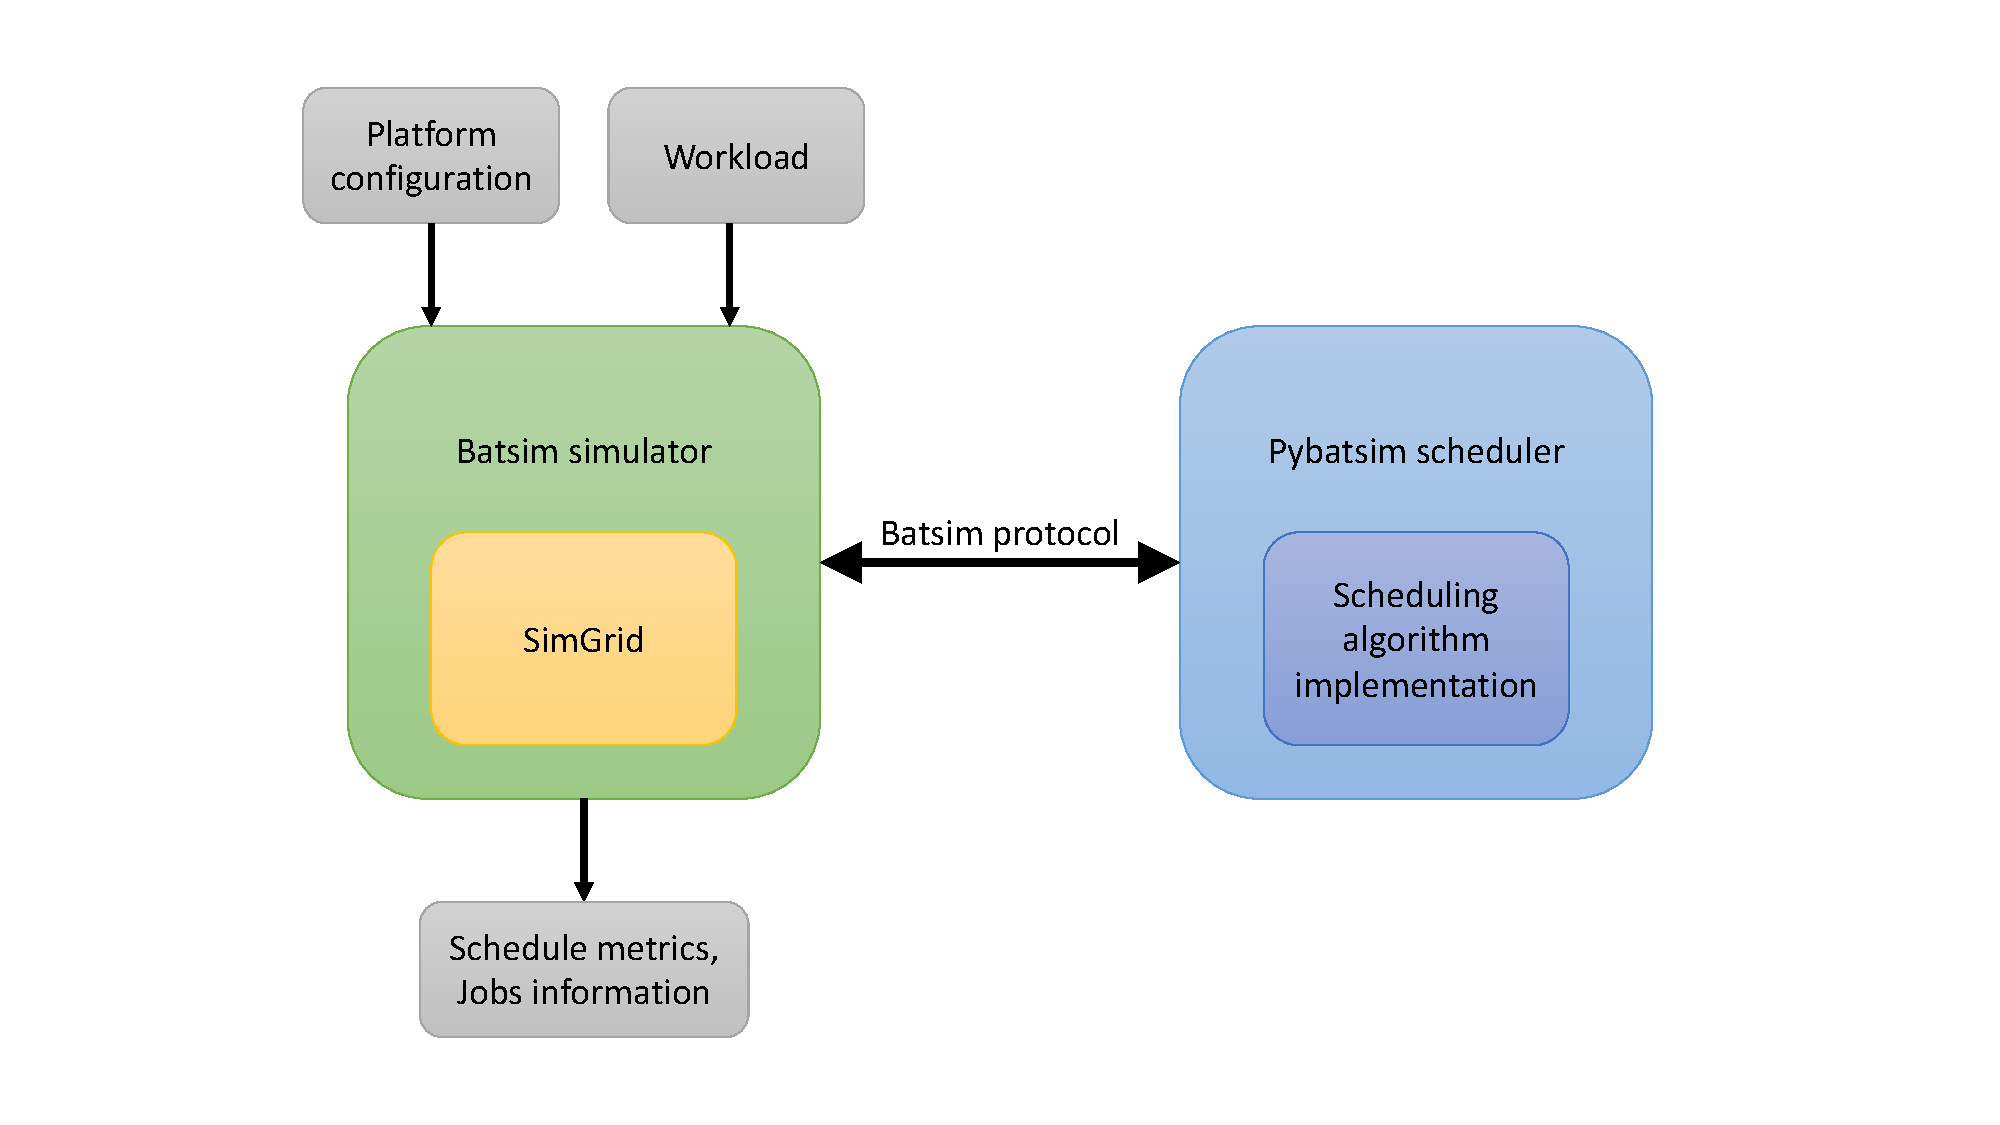
\includegraphics[width=\textwidth]{images/Batsim-architecture.pdf}
    \caption{Key components of the Batsim architecture from a user perspective}
    \label{fig:batsim-architecture}
\end{figure}

% The Batsim architecture in comparison with a real RJMS is shown in \autoref{fig:batsim}.
% \begin{figure}[ht]
%     \centering
%     \includesvg[inkscapelatex=false,width=\textwidth]{images/batsim_rjms_overview}
%     \captionsource{Comparison of a real RJMS with the Batsim architecture: scheduler process (decision maker) and simulator process (batsim). The platform simulation is performed by SimGrid.}
%     {\url{https://gitlab.inria.fr/batsim/batsim/-/blob/master/docs/img/batsim_rjms_overview.svg}}
%     \label{fig:batsim}
% \end{figure}

\bigskip

Yet another simulator that could support burst buffer related research is CODES \cite{codes,Cope2011CODESEC,osti_1311761}. This simulator was developed to explore the design of exascale storage architectures and distributed data-intensive science facilities. It is focused on the fine-grained simulation of I/O workloads in high-performance environments. A number of research publications regarding burst buffers have been already carried with CODES \cite{6232369,10.1145/2832087.2832091,8048932}.

However, for the research of batch scheduling, we find the higher-level simulation offered by Batsim to be a more suitable approach.

\subsection{Pybatsim}
Batsim is provided with four projects in C++, Python, D and Rust implementing the Batsim protocol on the scheduling side. For this dissertation, the Python implementation, named Pybatsim \cite{pybatsim-repo}, was chosen as an origin for implementation of our burst buffers aware scheduler.

Pybatsim exposes low and high-level APIs. The low-level API is merely a wrapper of the Batsim protocol that provides a set of callbacks and functions to interact with the simulator. The high-level API wraps the low-level API and offers numerous functions useful for implementation of basic scheduling algorithms, but at the cost of higher code complexity.

\section{Parallel Workloads Archive} \label{sec:archive}
The source of workloads for our performed experiments is the Parallel Workloads Archive \cite{FEITELSON20142967, parallel-workload-archive}, which is an \href{https://www.cs.huji.ac.il/labs/parallel/workload/}{online archive} that contains normalised logs of batch workloads gathered from various supercomputers, clusters and grids. It also includes a selection of parallel workload models derived from those logs.

The logs are stored as text files in the Standard Workload Format (SWF), which is essentially the CSV file format extended with comments in the preamble. A single entry in an SWF file is a description of a job that was executed in a given parallel system. The content and order of the SWF entry is described in detail in \cite{10.5555/2808941}. Below, we present a list of the fields which were used in our research together with their original description.
\medskip
\begin{itemize}
\item \textbf{Job number}: a counter field, starting from 1.
\item \textbf{Submit time} in seconds, relative to the start of the log.
\item \textbf{Runtime} (wallclock) in seconds. “Wait time” and “runtime” are used instead of the equivalent “start time” and “end time” because they are directly attributable to the scheduler and application, and are also suitable for models where only the runtime is relevant.
\item \textbf{Requested number of processors}.
\item \textbf{Requested runtime} (or CPU time).
\item \textbf{Requested memory} (again kilobytes per processor).
\end{itemize}

The job number and submit time were shifted to $0$ on conversion from SWF to the Batsim workload format. In \autoref{sec:bbrequest}, we investigated a correlation between the requested number of processors and requested memory. Therefore, we created a burst buffer request model using the requested memory field. Lastly, the runtime field and the requested runtime (walltime), together with the created model, were used to generate the Batsim workload, which in detail is described in \autoref{sec:workload}.
\end{document}